% Shared standalone design for the editable figure reconstructions.
\documentclass[tikz,border=5pt,10pt]{standalone}
\usepackage[T1]{fontenc}
\usepackage[utf8]{inputenc}
\usepackage{newpxtext,newpxmath}
\usepackage[scaled=.94]{sourcesanspro}
\usepackage{pgfplots}
\pgfplotsset{compat=1.18}
\usetikzlibrary{arrows.meta,calc,positioning,decorations.pathreplacing,
  decorations.markings,patterns,matrix,shapes.geometric,fit,backgrounds,
  intersections,angles,quotes}
\definecolor{ink}{HTML}{203746}
\definecolor{accent}{HTML}{146C78}
\definecolor{muted}{HTML}{667780}
\definecolor{signalred}{HTML}{B94B44}
\color{ink}
\tikzset{>=Latex,line width=.8pt,
  every node/.style={font=\small},
  axis/.style={->,draw=muted,line width=.5pt},
  guide/.style={draw=muted,dashed,line width=.45pt},
  curve/.style={draw=accent,line width=1pt},
  marker/.style={circle,fill=accent,inner sep=1.5pt},
  labelbox/.style={fill=white,inner sep=2pt}}

\begin{document}
\begin{tikzpicture}
\path[use as bounding box] (-.6,-.95) rectangle (10.8,5.4);
\draw[axis] (0,0)--(9.5,0) node[right] {$z$};
\draw[signalred,dashed] plot[domain=.8:8.0,samples=101] (\x,{1.4+.22*(\x-4.1)+.15*(\x-4.1)^2});
\draw[curve] plot[domain=.8:8.0,samples=101] (\x,{1.4+.22*(\x-4.1)+.105*(\x-4.1)^2});
\draw[muted,dashed] plot[domain=.8:8.0,samples=101] (\x,{1.4+.22*(\x-4.1)+.055*(\x-4.1)^2});
\draw[ink,line width=.6pt] (.7,.652)--(8.7,2.412);
\fill[ink] (4.1,1.4) circle (1.8pt);\draw[guide] (4.1,0)--(4.1,1.4);\node[below] at (4.1,0) {$x$};
\node[signalred,anchor=west] at (8.1,4.5395) {$Q_L(z)$};\node[accent,anchor=west] at (8.1,3.85505) {$f(z)$};\node[muted,anchor=west] at (8.1,3.09455) {$Q_\mu(z)$};
\node at (4.8,5.05) {$Q_\mu(z)\leq f(z)\leq Q_L(z)$};
\node at (4.8,-.55) {$Q_a(z)=f(x)+\langle\nabla f(x),z-x\rangle+\tfrac a2\|z-x\|^2$};
\end{tikzpicture}
\end{document}
